\begin{block}{Parameter Identification}
\centering
        \heading{Goal: Obtain the Best Value of $\lambda$} 
            {\large \textbf{Bayesian Context:} Regular Bayes model uses assumed likelihood function of data given $\lambda$.}
            
            {\large \textbf{Data Consistent Context:} Uses data to construct a predicted distribution of the average residuals given $\lambda$.}
            
            %{\large How do we update initial descriptions of uncertainty using model predictions and data?}

        %\heading{Background}
             %{\large \emph{Data Consistent Inversion} is a Measure-Theoretic Framework for the solution of stochastic inverse problems. }
             %{\large \textbf{Data-Consistent Inversion} is a novel framework that uses push-forward and pull-back measures to ensure solutions are consistent with the observed distribution of data.}

        %\heading{Question} 
          %   {\large \emph{How do we cast a \textbf{Parameter Identification} problem in the context of Data-Consistent Inversion?} }

\end{block}

\vspace{-0.75cm}
\begin{block}{Example}
\centering
    Consider an exponential decay problem with uncertain decay rate:
   \begin{equation*}
       u(t) = u_0\exp(-\lambda t), \; u_0 = 0.5 ,\; t\in[0,3]
   \end{equation*}
\vspace{-0.5cm}
    \begin{figure}
        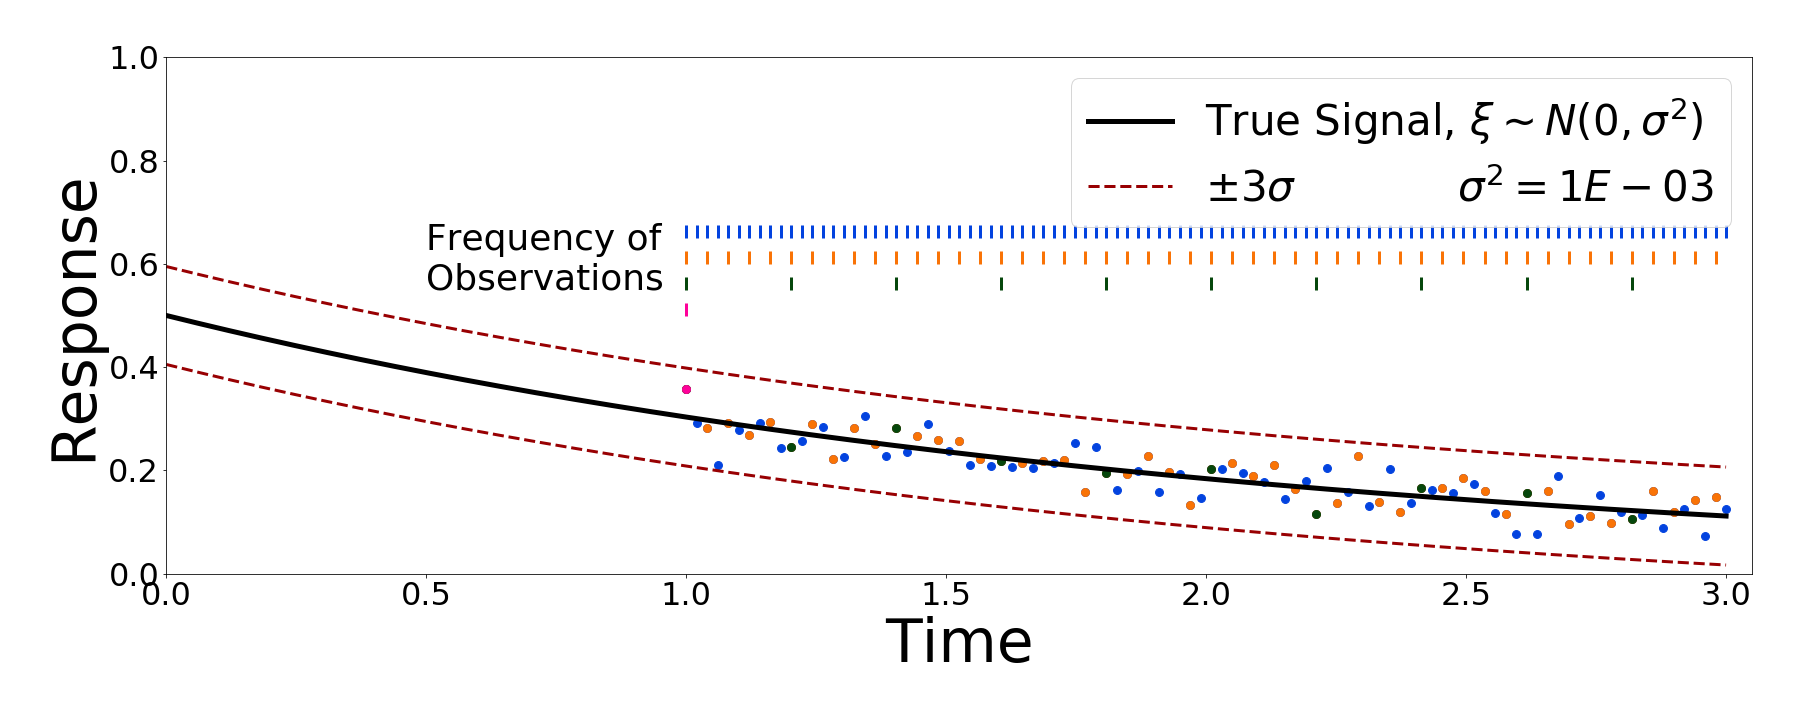
\includegraphics[width=26cm]{figures/exponential_decay_response_sigma-10E-4}
    \end{figure}

%\end{block}

\vspace{-0.5cm}

%\begin{block}{Convergence}
\centering
\heading{Convergence of Data Consistent Inversion}
{\emph How do solutions change with more data?}
\vspace{-0.5cm}
    \begin{figure}
        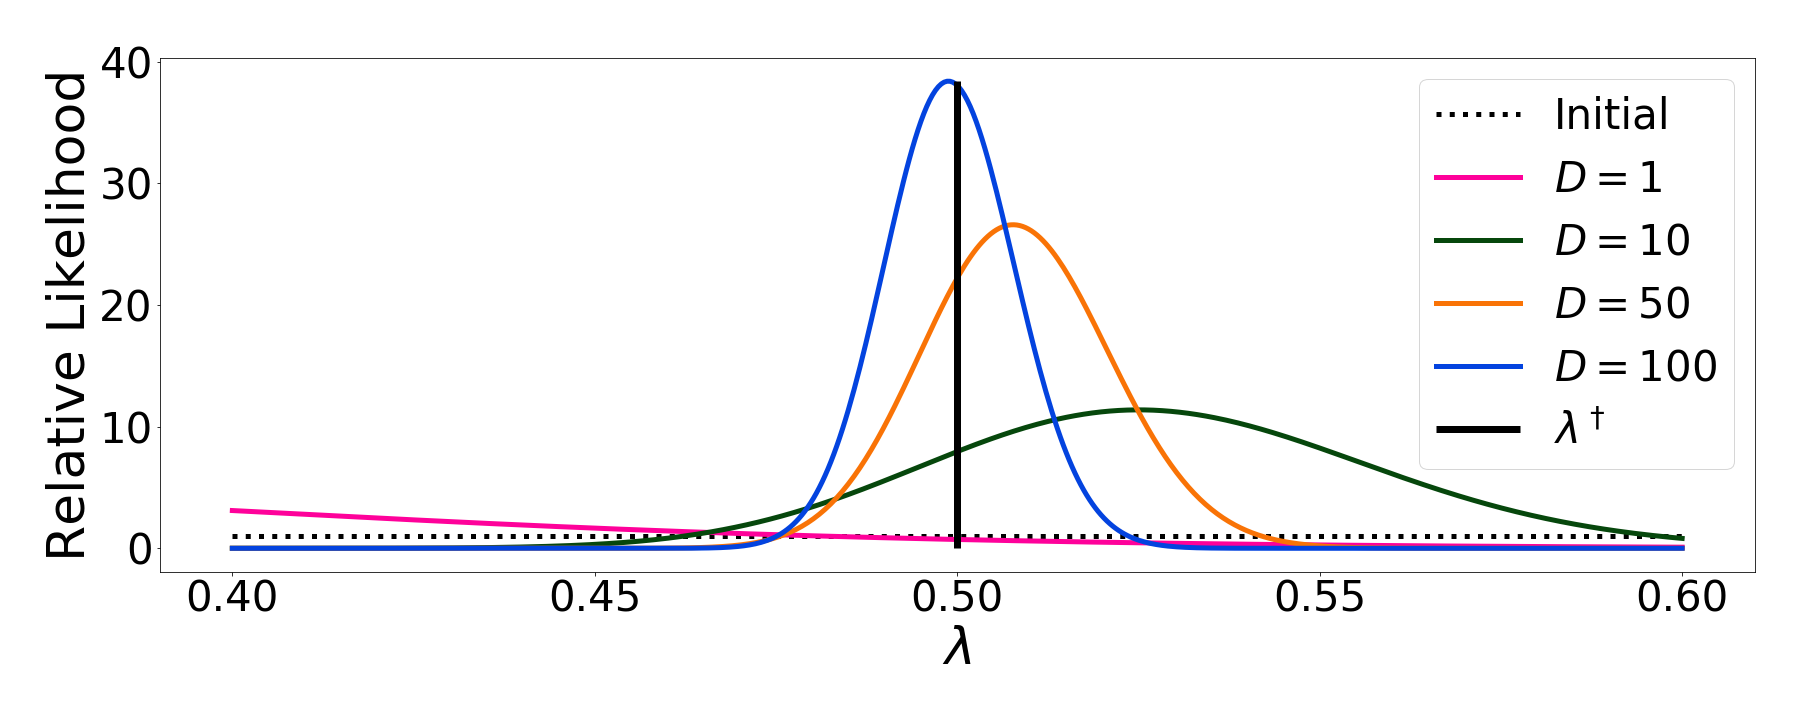
\includegraphics[width=26cm]{figures/updated_convergence_sigma-10E-4}
        \vspace{-0.5cm}
        \caption{ $\param^\dagger$ and $\updated$ for $D=1, 10, 50, 100$ for $N=1000$}
    \end{figure}

%\end{block}

\vspace{-0.5cm}

%\begin{block}{Stability}
\heading{Comparison to Regular Bayes}
{\emph How do solutions on conditionals of $\nspace$ compare?}
\vspace{-0.5cm}
    \begin{figure}
        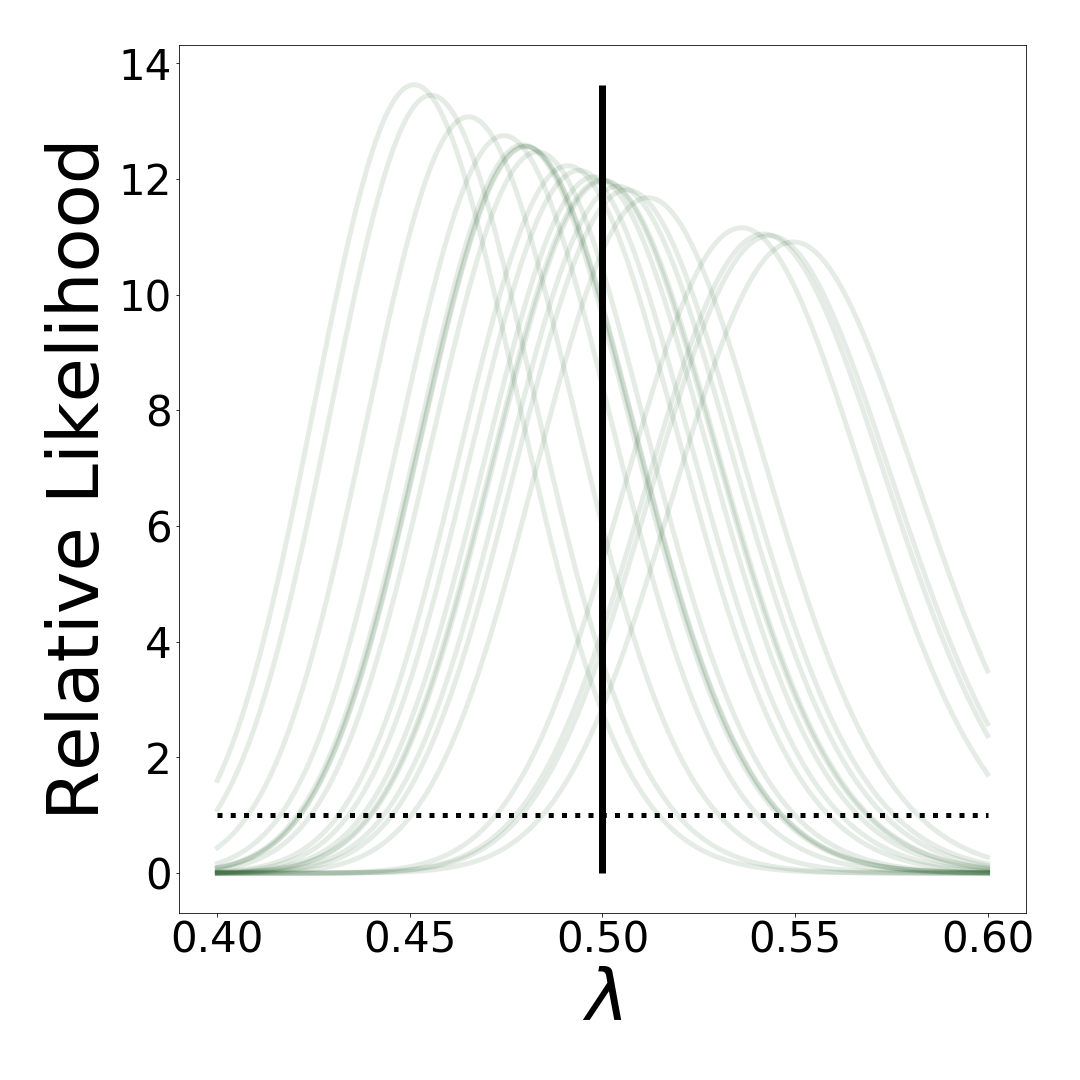
\includegraphics[width=13cm]{figures/updated_stability_D10_sigma-10E-4}
        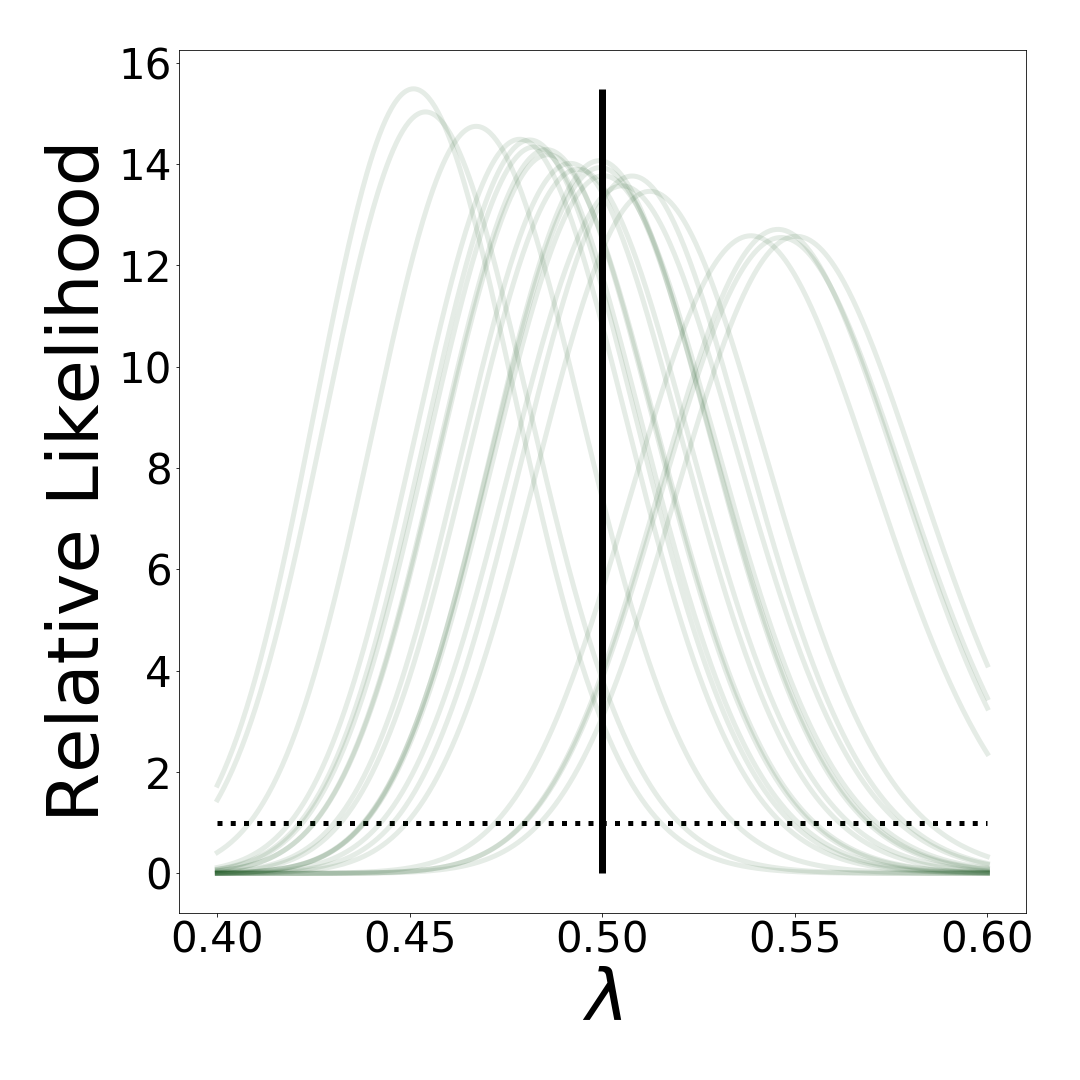
\includegraphics[width=13cm]{figures/posterior_stability_D10_sigma-10E-4}\\
        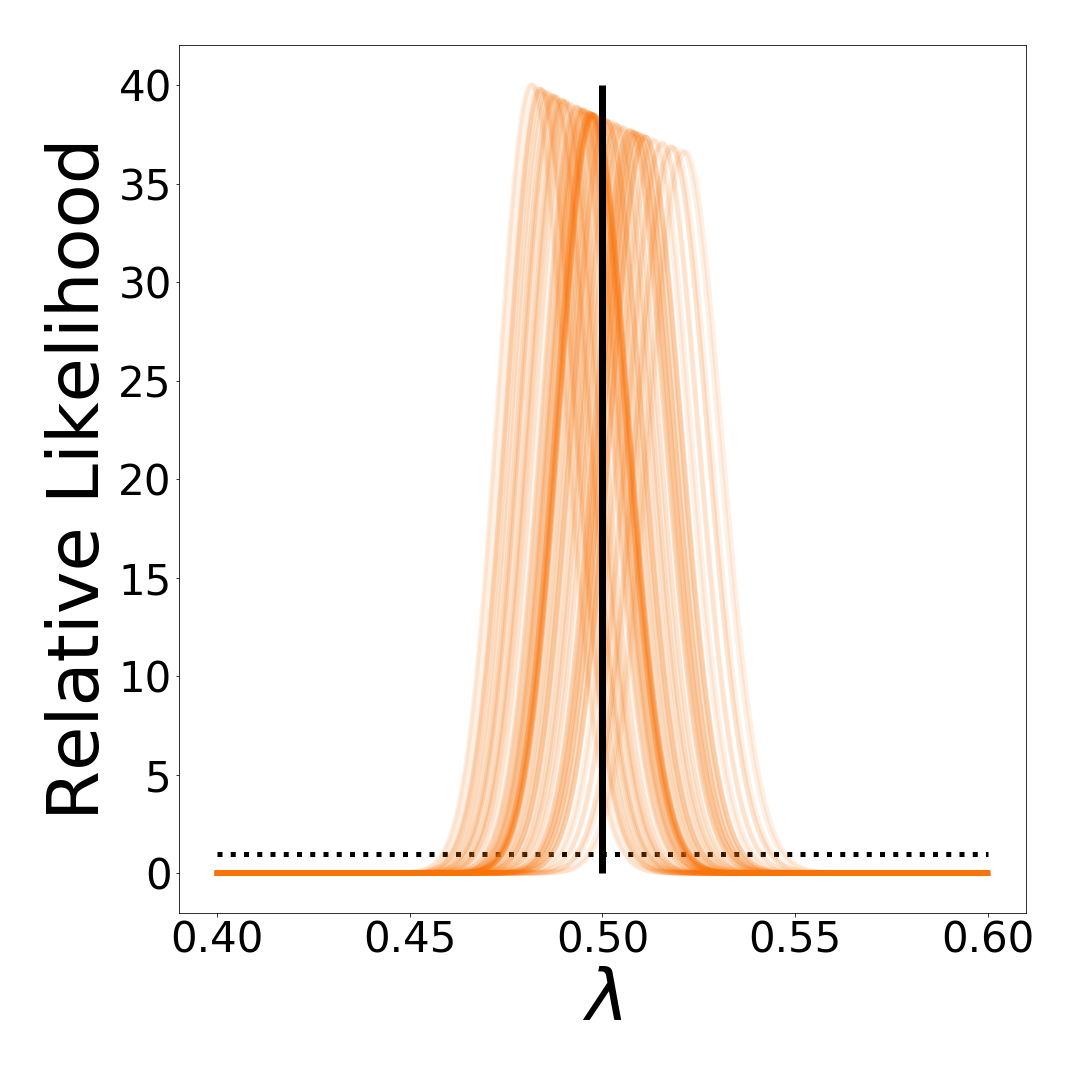
\includegraphics[width=13cm]{figures/updated_stability_D100_sigma-10E-4}
        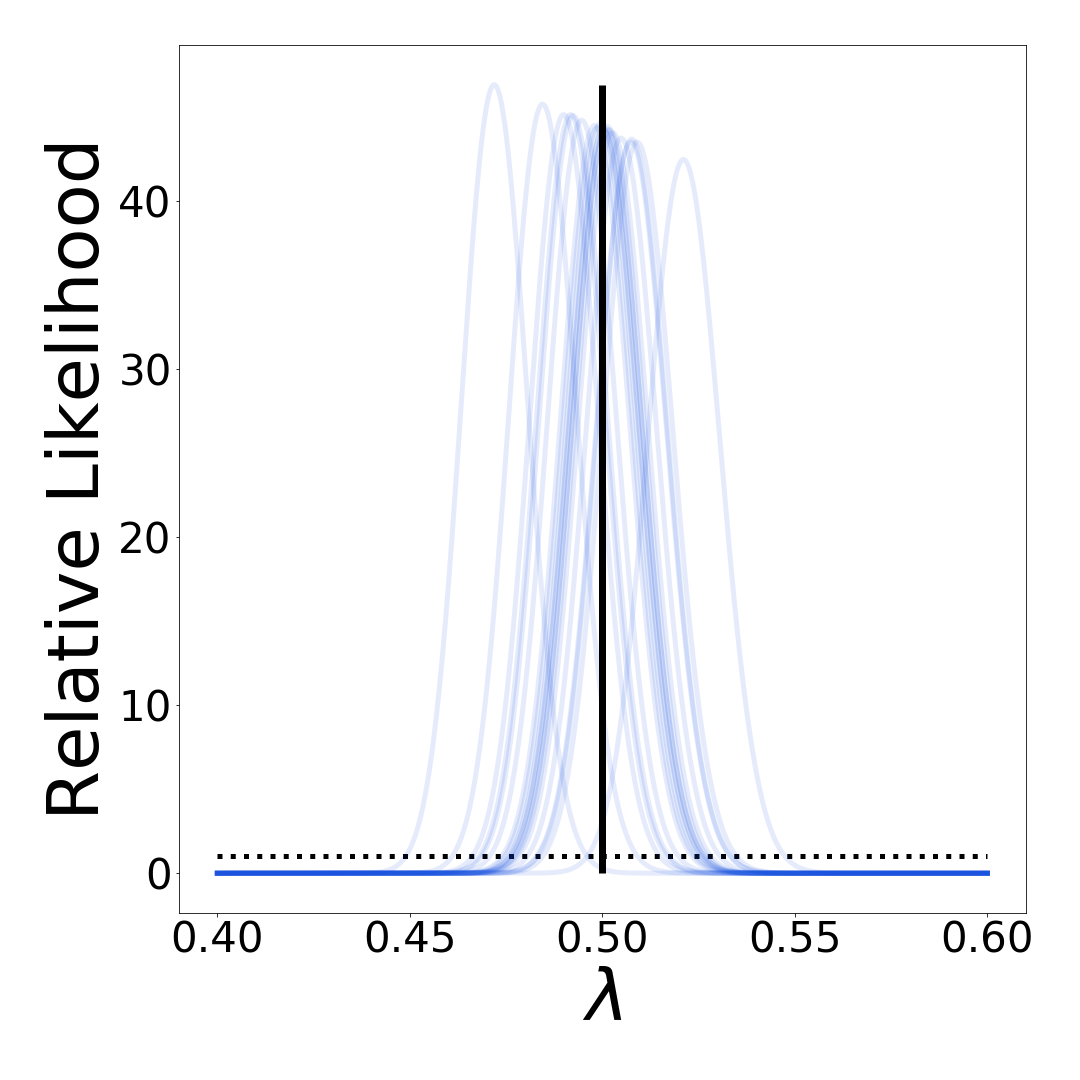
\includegraphics[width=13cm]{figures/posterior_stability_D100_sigma-10E-4}
        \vspace{-1cm}
        \caption{100 realizations of $\noise^\dagger$ for $D=10,100$ for Data-Consistent Inversion (left) and Regular Bayes (right).}
    \end{figure}

\end{block}
